\section{Introduction}\label{sec:introduction}

In the combinatorial integral approximation (CIA) decomposition of
mixed-integer optimal control~\cite{sager2011cia}, a relaxed control that may
divide activity among several modes is rounded to an integer control that
activates one mode at a time. The rounding error is the largest absolute
difference between the cumulative mode allocations of the two controls; under
regularity assumptions it bounds the resulting state
error~\cite{sager2011cia,zeile2022decomposition}. Without switching
restrictions, sum-up rounding makes this error proportional to the grid width,
so it vanishes under refinement~\cite{sager2011cia,kirches2020tight}. With a
hard bound on the number of switches it does not~\cite{sager-zeile2021}:
refinement only improves the placement of finitely many switches and cannot
remove the error caused by the budget itself. The relevant questions are
therefore quantitative: what error is unavoidable, which relaxed inputs attain
it, and how can one compute an optimal or certifiably near-optimal schedule
for a given input?

We answer these questions for measurable simplex-valued controls on a horizon
$[0,T]$, with $n$ modes and at most $s$ switches, that is, at most $k=s+1$
activation blocks. The initial mode is free, repeated modes are allowed, and
the default model has no dwell or transition restrictions. For an input
cumulative allocation $A$, write $\OPT_s(A)$ for the smallest cumulative
discrepancy among continuous-time schedules and $F_{n,s}(T)=\max_A\OPT_s(A)$
for its worst-case value. A superscript $\mathcal T$ restricts switching times
to a grid $\mathcal T$.

\subsection{Main results}

\paragraph{Sharp continuous minimax values.}
Our main formula (Theorem~\ref{thm:small-full}) is
\begin{equation}\label{eq:intro-main}
 F_{n,s}(T)=T\max\left\{\frac{1}{s+2},
 \frac{1}{n\bigl((n/(n-1))^{s+1}-1\bigr)}\right\},
 \qquad 0\le s\le3,\quad n\ge s+2.
\end{equation}
The first term is attained by $s+2$ successive pure modes of equal duration.
The second is the sharp one-sided error of the uniform input on all $n$
modes. It exceeds the first from $n=5,8,12$ onward for $s=1,2,3$,
respectively (Figure~\ref{fig:minimax-regimes}). Thus the continuous lower
bound $T/(s+2)$ of Sager and Zeile~\cite[Proposition~4]{sager-zeile2021} is
the exact value for $s+2\le n\le4,7,11$ and is exceeded for larger $n$,
contrary to their remark that this bound cannot be
improved~\cite[p.~615]{sager-zeile2021}. The
formula covers all measurable inputs, and its lower bound allows competing
schedules to repeat modes.

\begin{figure}[tb]
\centering
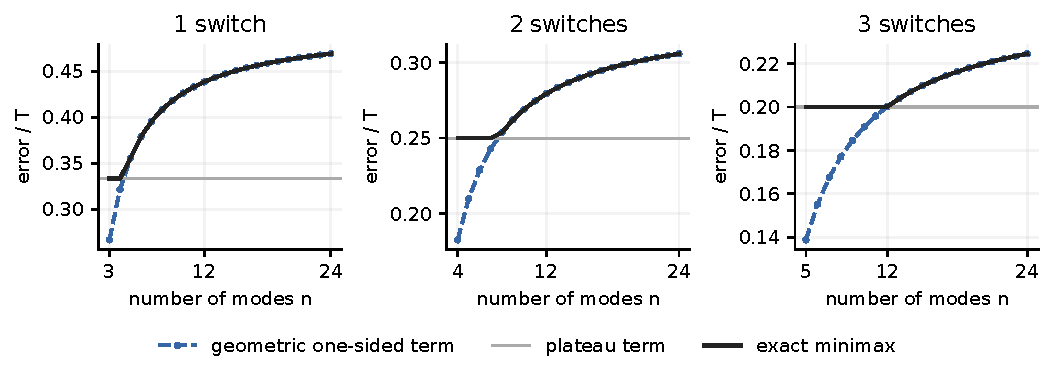
\includegraphics[width=\linewidth]{figures/minimax-regimes.pdf}
\caption{The exact continuous minimax value divided by $T$, its plateau term, and
the geometric one-sided uniform term
for one, two, and three switches, on their stated mode ranges. Lines connect
integer mode counts.}
\label{fig:minimax-regimes}
\end{figure}

The proof separates heavy modes from a one-sided problem. If some terminal
mode mass exceeds $E$ and $T\le(s+2)E$, integral-prefix rounding followed by
a reordering at the first repeated mode gives an $s$-switch schedule with
full error at most $E$, for every $n$ (Theorem~\ref{thm:heavy}). Otherwise
only the one-sided error matters (Theorem~\ref{thm:one-sided-reduction}),
and we prove sharp reach bounds for schedules with up to four distinct modes.
The two- and three-block arguments are analytic
(Lemma~\ref{lem:reach-two}, Theorem~\ref{thm:reach-three}); the four-block
bound (Theorem~\ref{thm:reach-four}) is computer-assisted, using exact
rational and polynomial dual certificates for a necessary-condition linear
program after a symmetry reduction, for every $n\ge5$. The spare-mode
hypothesis $n>k$ cannot simply be dropped: at $n=k=3$ a constructed input
has an exact three-block one-sided optimum strictly worse than the uniform
input, even when modes may repeat (Proposition~\ref{prop:three-mode-failure}).

\paragraph{General budgets.}
For every $k=s+1<n$, removing a largest-mass or a smallest-mass mode carries
one-sided bounds from $n-1$ modes and $k-1$ blocks to $n$ modes and $k$
blocks (Lemma~\ref{lem:mode-removal}).
This gives a closed upper coefficient (Theorem~\ref{thm:general-coefficient}),
a sharper bound seeded by the four-block theorem (Theorem~\ref{thm:seeded}),
the plateau value $F_{n,k-1}(T)=T/(k+1)$ at least for
$k+1\le n\le\max\{2k,k(k+1)/2\}$ (Corollaries~\ref{cor:general-plateau}
and~\ref{cor:light-boundaries}), and
\[
 F_{n,k-1}(T)=\frac{T}{k}-\frac{(k+1)T}{2kn}
                  +O_k(Tn^{-2})\qquad(n\to\infty)
\]
(Proposition~\ref{prop:general-asymptotics}). The leading dimension-free
term $T/k$ already follows from classical integral-prefix rounding
(Proposition~\ref{prop:dimension-free}); the first mode-count correction is
sharp. Inputs with equal terminal masses have stronger guarantees, including
the exact instance value $T/n$ in a band next to $n=k$
(Corollary~\ref{cor:light-boundaries}). The exact reach bound for five or
more blocks remains open; Appendix~\ref{sec:higher-reach} isolates the
missing inequality, and no other result depends on it.

\paragraph{Exact finite-grid values.}
On an arbitrary grid with $N$ cells and $n\ge3$, the one-switch minimax value
is an explicit maximum over $O(N^2)$ closed-form candidates, evaluable in
$O(N^2)$ rational operations for rational grid data; a worst input has two
component types and at most three time phases
(Theorem~\ref{thm:finite-one}). For three modes on
unit grids, a complete description of the realizable floor histories
(Proposition~\ref{prop:floor-automaton}), valid for every grid length, gives
exact values on five, six, and seven cells
(Theorems~\ref{thm:five-cells} and~\ref{thm:seven-cells},
Corollary~\ref{cor:six-cells}), including
$F^{\mathrm{unit}}_{3,3}(7)=4/3$. The five- and six-cell values give the
upper bounds in $F_{3,2}(T)=T/5$ (Corollary~\ref{cor:three-two-continuous})
and $T/7\le F_{3,3}(T)\le T/6$; the lower bounds are the case $n=3$ of
\cite[Proposition~4]{sager-zeile2021}. The exact value of $F_{3,3}$ remains
open. Together with the uniform-input examples of
Section~\ref{sec:one-switch}, these results disprove three specific
finite-grid statements of \citet{sager-zeile2021}: the first branch of their
Conjecture~1 fails even as an upper bound
(Examples~\ref{ex:five-mode-conjecture} and~\ref{ex:three-cell-conjecture}),
the equality in its second branch fails on seven cells, and the lower bound
in their Corollary~5 fails on five cells
(Section~\ref{sec:floor-chambers}).

\paragraph{Exact algorithms for a given input.}
For a supplied input on $N$ grid cells, three candidate mode pairs per grid
boundary suffice for one switch, which gives an exact $O(nN)$ algorithm
(Theorem~\ref{thm:linear-one-switch}). For a fixed budget, enumerating the
block boundaries and assigning blocks to modes by a subset dynamic program
gives an exact algorithm whose arithmetic cost is polynomial in $N$ for each
fixed $s$ and linear in $n$ (Theorem~\ref{thm:fixed-budget}). It allows
repeated modes and can enforce mode-specific minimum dwell times on maximal
runs. For piecewise-affine input and switches anywhere in time, a finite
family of rational linear programs gives the continuous instance optimum
exactly (Section~\ref{sec:algorithms}).

\paragraph{Sharp grid transfer and certified coarsening.}
A chronological, support-preserving rounding moves any finitely switching
schedule to a uniform grid of width $h$ without adding switches and changes
cumulative occupations by strictly less than $h$
(Theorem~\ref{thm:sharp-transfer}). Hence
$\OPT_s(A)\le\OPT^{\mathcal T}_s(A)<\OPT_s(A)+h$, with the analogous
minimax inequality (Corollary~\ref{cor:opt-transfer}); the coefficient one
is sharp uniformly over modes and budgets
(Proposition~\ref{prop:transfer-sharpness}). Exact optimization on a coarse
uniform grid therefore returns a feasible schedule together with a certified
additive interval for the continuous optimum
(Theorem~\ref{thm:certified-coarsening}), with explicit bounds for input
quantization (Corollary~\ref{cor:coarse-perturbation}). Dwell constraints
need separate treatment: an elementary example keeps a fixed positive gap on
arbitrarily fine odd grids (Example~\ref{ex:dwell-grid-gap}).

\paragraph{Computations and verification.}
Section~\ref{sec:computations} applies these methods in exact rational
arithmetic to a public three-mode Lotka--Volterra relaxed control on 12,000
cells~\cite{pycombina-data}. For the quantized input, the exact one-switch
optimum on the full grid is $1.889$, against the continuous optimum
$1.8885876$, and a 48-cell coarse grid brackets the continuous three-switch
optimum in an interval of width $0.25$. Separate Lean developments verify the arbitrary-grid one-switch formula, the transfer and
coarsening results with their supporting instance algorithms, the exact
five-, six-, and seven-cell three-mode values, and $F_{3,2}(T)=T/5$;
Section~\ref{sec:discussion} states their scope.

\begin{table}[tb]
\centering\small
\caption{Main scopes. Here $k=s+1$, and a unit grid has horizon $N$.}
\label{tab:results-synopsis}
\begin{tabular}{@{}p{.32\linewidth}p{.43\linewidth}p{.18\linewidth}@{}}
\toprule
Problem & Result & Reference\\
\midrule
Continuous minimax, $0\le s\le3$, $n\ge s+2$
 & Exact formula~\eqref{eq:intro-main} & Theorem~\ref{thm:small-full}\\
General budgets, $n>k$ & Closed and seeded upper bounds; sharp first correction
 & Section~\ref{sec:general-budgets}\\
Three-mode boundaries & $F_{3,2}=T/5$; $T/7\le F_{3,3}\le T/6$
 & Section~\ref{sec:floor-chambers}\\
One-switch grid minimax, $n\ge3$ & Explicit formula on arbitrary grids
 & Theorem~\ref{thm:finite-one}\\
Three-mode unit grids & $(N,s)=(5,2),(6,3),(7,3)$: values $1,1,4/3$
 & Section~\ref{sec:floor-chambers}\\
Supplied grid input & Exact one-switch and fixed-budget algorithms
 & Section~\ref{sec:algorithms}\\
Continuous-to-grid transfer & Sharp uniform coefficient; additive certificates
 & Section~\ref{sec:transfer}\\
\bottomrule
\end{tabular}
\end{table}

\subsection{Relation to earlier work}

Sager, Jung, and Kirches~\cite{sager2011cia} introduced the CIA decomposition
and the switch-constrained rounding subproblem, with a mixed-integer linear
formulation and a tailored branch-and-bound algorithm. Sager and
Zeile~\cite{sager-zeile2021} study a total-variation constraint on the
integer control, develop maximum dwell rounding, and give the worst-case
bounds and conjecture compared above; Sections~\ref{sec:one-switch}
and~\ref{sec:floor-chambers} compare their finite-grid statements in
detail.

Integral flow and matching are established tools for rounding partial sums;
Knuth's two-way rounding theorem~\cite{knuth1995} is a classical example.
Bestehorn and Kirches~\cite[Corollary~2.7]{bestehorn2021vanishing} prove
support-preserving CIA rounding with discrepancy at most one uniform grid
width. Our transfer proof gives this construction explicitly and adds the
chronological argument that preserves a supplied schedule's switch count,
the strict bound, and a sharp instance-wise discretization family.
Section~\ref{sec:transfer} also gives a counterexample to the unrestricted
instance-wise reading of the half-grid argument preceding their
Conjecture~1~\cite[p.~615]{sager-zeile2021} (see also
\cite[p.~139]{zeile2021thesis}), which is not stated as a theorem.

Exact graph algorithms for switching costs, minimum dwell times, and support
restrictions already exist. The shortest-path formulation of Bestehorn,
Hansknecht, Kirches, and Manns~\cite{bestehorn2021shortest} gives
switching-cost-aware rounding (SCARP), with a complexity bound exponential in
the mode count. Zeile, Robuschi, and Sager~\cite{zeile2021dwell} analyze
minimum dwell rounding, and switching-time enumeration is discussed in
\cite[Section~6.4.3]{zeile2021thesis}. Abbasi-Esfeden, Plate, Sager, and
Swevers~\cite{abbasi2025} propose a dynamic-programming-inspired CIA method
with dwell constraints; they state that it does not guarantee global
optimality in general, because optimal substructure is lost. What is
specific to our exact algorithms is the CIA dominance and subset reduction,
with its proved linear dependence on the mode count for a fixed budget.

Several approximation results concern grids whose refinement lets the number
of switches grow: tight sum-up rounding bounds~\cite{kirches2020tight},
compactness and convergence of CIA decompositions~\cite{kirches2021compact},
and adaptive nonuniform refinement for SCARP~\cite{bestehorn2023adaptive}.
Our coarsening certificate instead concerns the best approximation under a
fixed switch budget, to a prescribed additive accuracy, including exact
integration across nonaligned input and output grids. It does not assert
convergence to the relaxed control at fixed budget. Our results concern
discrepancy, switching feasibility, and computational cost only;
consequences for states or objectives of an underlying control problem
require its dynamics and the regularity assumptions of
\cite[Theorem~1 and Corollary~1]{zeile2022decomposition}.

\subsection{Organization}

Section~\ref{sec:foundations} defines the model.
Sections~\ref{sec:one-switch}--\ref{sec:structural-limits} prove the
continuous results through three switches and show where the constructions
stop, and Sections~\ref{sec:general-budgets}--\ref{sec:predecessors} treat
general budgets. Sections~\ref{sec:finite-one}--\ref{sec:floor-chambers}
give the finite-grid values, Sections~\ref{sec:algorithms}
and~\ref{sec:transfer} the instance algorithms and certificates, and
Section~\ref{sec:computations} the computations.
Section~\ref{sec:discussion} discusses open questions;
Appendix~\ref{sec:higher-reach} treats the higher-reach question.
